%\documentclass[letterpaper, 10pt]{sigcomm-alternate}

% \documentclass[peerreview, a4paper, draft, 7pt]{IEEEtran}
\documentclass[a4paper, 10pt]{IEEEtran}
\usepackage{times}
%\usepackage{color}
% \usepackage{caption2}
\usepackage{subfigure}
\usepackage{graphicx}
\usepackage{colortbl}
\usepackage[dvipsnames]{xcolor}
% \usepackage{ulem}

\pagenumbering{arabic}

\ifx\pdfoutput\undefined
\usepackage[pdfpagemode=none, pdfstartview=FitH, colorlinks=true, urlcolor=black, linkcolor=black, citecolor=black, letterpaper]{hyperref}
\else
\usepackage[pdftex, pdfpagemode=none, pdfstartview=FitH, colorlinks=true, urlcolor=black, linkcolor=black, citecolor=black, letterpaper, pdftex]{hyperref}
\fi

%% Editorial work
% \newcommand{\purge}[1]{\textcolor{red}{\sout{#1}}}
% \newcommand{\add}[1]{\textcolor{blue}{#1}}

%%% End of editorial work.


 
\renewcommand{\em}[1]{\textit{#1}}
\begin{document}

\title{Smart Objects Security: Considerations for Transport Layer Security Implementations}

\author{\authorblockN{Hannes Tschofenig\authorrefmark{1}\\}
\authorblockA{\authorrefmark{1}Nokia Siemens Networks, 
Email: Hannes.Tschofenig@nsn.com\\}
\thanks{\textsc{
Position paper for the 'Smart Object Security' workshop, Friday, 23rd March 2012, Paris. This paper represents the views of the author in his role as an individual contributor to the Internet standards process. They do not reflect the consensus of the Internet Engineering Task Force (IETF) at large, of any IETF working group, or of the Internet Architecture Board (IAB). Referenced documents may, however, reflect IETF consensus. The author is a member of the IAB and has contributed to the standardization efforts discussed in this document.}}
}

\date{\today}

\maketitle

\section{Abstract}

Transport Layer Security (TLS) is a widely uses security protocol that offers a range of security services on top of the transport layer. While the initial design had of TLS had focused on the protection of applications running on top of the Transmission Control Protocol (TCP), and used with the Hypertext Transfer Protocol (HTTP) in particular, subsequent standardized extensions also introduced support for User Datagram Protocol (UDP), Datagram Congestion Control Protocol (DCCP), and Stream Control Transmission Protocol (SCTP). The design of TLS is in the meanwhile classical for many security protocols - it separates the authentication and key exchange phase from the actual protection of the application data exchange. The same design pattern can also be found in many other security protocols, including the Internet Key Exchange protocol version 2 (IKEv2) and the IP security protocol suite. 

TLS is often seen as an inadequate choice for smart object deployments due to its perceived complexity. Such a statement is in general hard to justify absent a threat analysis and a list of security goals that need to be accomplished for a specific architecture. On top of this observation there is the challenge that smart objects may be constrained in various directions, such as flash and volatile memory limitations, energy and communication restrictions. An implementation that aims to fulfill the security goals in one specific environment may need to take a very different direction compared to one that targets a different environment. 

To offer input for implementers and system architects the author therefore illustrates the cost of various TLS features based on a selected lightweight implementation. Not surprisingly, every feature has a certain cost and tradeoff decisions need to be made. The writeup also looks at some recently proposed extensions. 

\section{Code Availability}

There are many reasons for reusing protocols develops by the Internet Engineering Task Force (IETF) and one reason relevant to this discussion is the widespread availability of high-quality open source code. Changes are good that there is already an open source TLS stack available for the target operating system running on a smart object. In such a case the integration effort is significant lower leading to a faster time to market and lower development costs. This is not an irrelevant factor in the design of smart object since costs are not only related to the hardware but also contributed by operating system and application development. 

A compilation of available TLS implementations can be found at \cite{TLS-Implementations}. While many of these implementations provide a good starting point for a developer the axTLS project \cite{axTLS} already claims to offer a small code footprint. Beyond these implementations there is also open source code with EAP-TLS, which is used for network access authentication. Unlike the previous implementations the code first needs to be decoupled from the EAP specific encapsulation. The WPA Supplicant \cite{wpa-supplicant} (for the client side) and the FreeRADIUS \cite{FreeRADIUS} (for the server side) contains TLS libraries that could be utilized -- the WPA Supplicant already provides the support for an internal crypto library that does not rely on libraries, like OpenSSL. 

The author had chosen axTLS and the remainder of the paper refers to that specific implementation. axTLS is a C-based implementation of TLS v1.0 and TLS v1.1 and offers the following features: 
\begin{itemize}
\item Certificate support (X509v1, self-signed certificates, PKCS\#8, PKCS\#12 keys/certificates in DER/PEM format, 
\item Certificate verification and identity checks, 
\item Session resumption,
\item Session renegotiation,
\item Various TLS Record Layer cipher algorithms: RC4-SHA1, AES128-SHA1, AES256-SHA1,  RC4-SHA1, RC4-MD5
\end{itemize}

TLS can easily be extended by adding new ciphersuites, if the large range of existing ciphersuites \cite{TLS-IANA} do not match the requirements. The axTLS implementation is focused on the support of ciphersuites that use RSA-based key transport and does not support TLS-PSK or Diffie-Hellman based key exchanges. DSA and ECC based public key based algorithms are not supported either. 

A very useful property of the axTLS library is the independence from other libraries. 

\section{TLS Introduction}

TBD: Text here. 

\begin{figure}[!t]
 \centering
 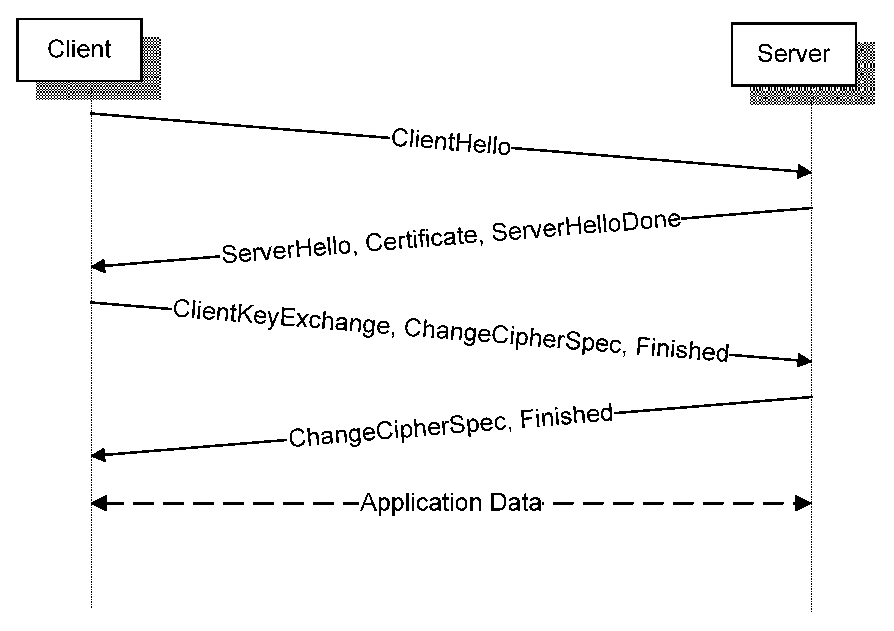
\includegraphics[scale=0.50]{TLS-Main-Exchange}
 \caption{TLS Exchange with Server-Only Authentication.}
 \label{tls-main-exchange-figure}
\end{figure}

TBD: Text here. 

\begin{figure}[!t]
 \centering
 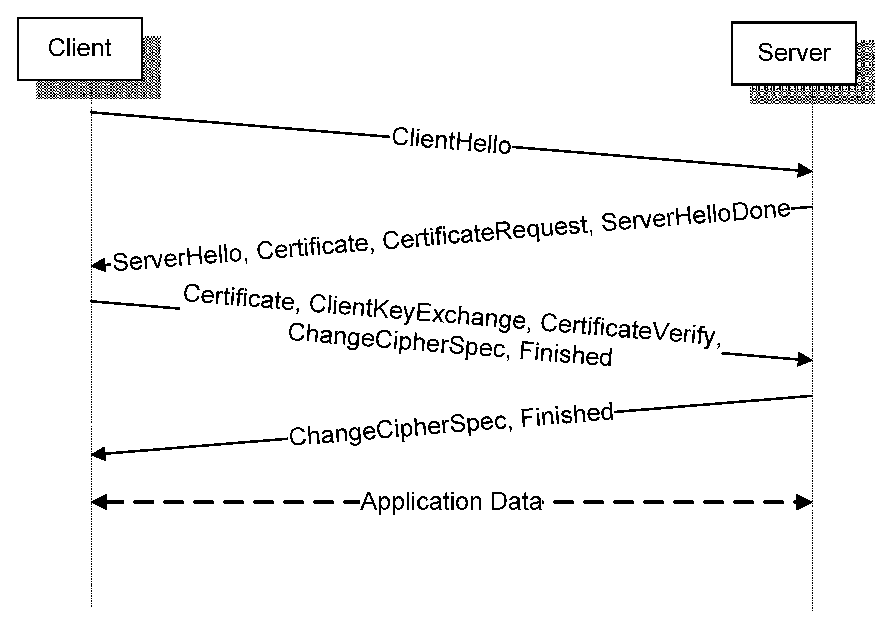
\includegraphics[scale=0.50]{TLS-Client-Authentication}
 \caption{TLS Exchange with Client and Server Authentication.}
 \label{tls-client-authentication-figure}
\end{figure}

TBD: Text here. 

\begin{figure}[!t]
 \centering
 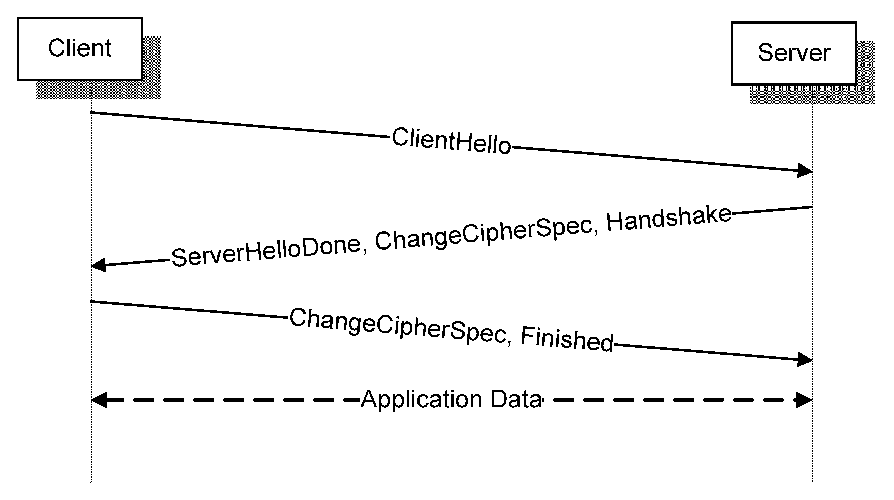
\includegraphics[scale=0.50]{TLS-Session-Resumption}
 \caption{TLS Session Resumption.}
 \label{tls-session-resumption-figure}
\end{figure}

\section{Communication Relationships}
\label{relationships} 

When designing a security solution the communication relationships need to be kept in mind. Consider the following scenario where a smart meter transmits its energy readings to other parties. The electricity will want to make sure that the obtained meter readings can be attributed to a specific meeting in a house hold. Most energy companies would find it unacceptable to have meter readings modified in transit (particularly changed to the disadvantage of the electricity provider since this would lead to fraud and a financial loss). Users in a house hold may want to ensure that only certain parties get to see the meter readings, for example for privacy reasons.  

In this example a sensor may need to only ever talk to servers of a specific electricity company or even to a single pre-configured server. Clearly, some information has to be pre-provisioned into the device to ensure the desired behavior to talk only to certain servers. The meter may be pre-provisioned with the domain name of the servers and with the root certificate that is used by the electricity company to sign certificates for their servers. The device may, however, also be configured to accept one or multiple server certificates. It may even be pre-provisioned with the server's raw public key, or a shared secret instead of relying on certificates. 

Lowering the flexibility decreases the implementation overhead. TLS-PSK \cite{rfc4279}, in case of shared secret usage, or raw public keys used with TLS \cite{I-d.ietf-tls-oob-pubkey} require fewer lines of code than x509 certificate usage, as it will be explained later in this document. A decision for constraining the client-side TLS implementation, for example by offering only a single ciphersuite, has to made in awareness of what functionality will be available on the TLS server-side. In certain communication environments it may be easy to influence both communication partners while in others cases the already deployed base needs to be considered. To illustrate the example, consider an Internet radio who allows a user to connect to available radio stations will be more constrained than an IP-enabled scale that connects only to the Web server offered by the manufacturer of that device. For the Internet radio case a threat assessment may most likely even conclude that TLS support is not necessary at all. 

Consider the following extension to our scenarios where the meter needs is attached to the households home WLAN network and WLAN specific security mechanisms may need to be taken care of. On top of the link layer authentication the previously explained application layer security mechanism needs to be implemented. Quite likely the security mechanisms will be different due to the different credential requirements. While there is a possibility for re-use of cryptographic libraries (such as the SHA1, MD5, HMAC code) the overall code footprint will be likely be larger. 

\section{Code Size}

One potential design goal is to reduce the size of the application code run on a smart object. To reduce the code size to a minimum it is crucial to understand the communication model and security goals, as explained in Section \ref{relationships}. Tradeoff decisions will have to be made consider the amount of flexibility and functionality offered by the TLS stack vs. the amount of required code that has to be run on a specific hardware platform. The following tables\footnote{The code was compiled under Debian Linux using -Os compiler flags for a 64-bit AMD machine. The same environment had been used for all other code compilations in this paper.} provide information about the code size of various security functions. 

\begin{table}[htdp]
\caption{Binary Code Size for Cryptography Support Functions}
\begin{center}
\begin{tabular}{|l|r|}
\hline
\textbf{Library} & \textbf{Code Size}\\
\hline\hline
MD5 & 5,552 bytes \\ 
\hline\hline
SHA1 & 3,392 bytes \\ 
\hline\hline
HMAC & 3,600 bytes \\
\hline\hline
RSA & 5,272 bytes \\
\hline\hline
Big Integer Implementation & 11,480 bytes \\ 
\hline\hline
AES & 7,096 bytes \\
% Compile AES code for illustrative purposes even though we do not make use of it. 
\hline\hline
RC4 & 2,232 bytes \\ 
\hline\hline
Random Number Generator & 6,232 bytes \\
% The crypto_misc.c file contains random number generator code as well as some other support functions. 
% Re-compile it to see how large it is with various debugging functions disabled. 
\hline
\end{tabular}
\end{center}
\label{crypto-code-table}
\end{table}

The library implementing the random number generator (RNG) allows OS support to be re-used but for the purpose of this illustration it had been disabled and therefore the RNG implementation is purely in software. A hardware platform that provides RNG support may likely lead to a smaller footprint. There are also other support functions that come with the C file (crypto\_misc.c) that contains the RNG  but those had been excluded with compile-time flags.

\begin{table}[htdp]
\caption{Binary Code Size for TLS-specific Code}
\begin{center}
\begin{tabular}{|p{1cm}|p{0,6cm}|p{5,8cm}|}
\hline
\textbf{Library Name} & \textbf{Code Size} & \textbf{Description} \\
\hline\hline
x509& 2,912 bytes & The x509 related code (\textit{x509.c}) provides functions to parse certificates, to copy them into the program internal data structures and to perform certificate related processing functions, like certificate verification.\\ 
\hline\hline
ASN1 Parser & 6,760 bytes & The ASN1 library (\textit{asn1.c}) contains the necessary code to parse ASN1 data.\\ 
\hline\hline
Generic TLS Library & 20,144 bytes & This library (\textit{tls1.c}) is separated from the TLS client specific code (\textit{tls1\_clnt.c}) to offer those functions that are common with the client and the server-side implementation. This includes code for the master secret generation, certificate validation and identity verification, computing the finished message, ciphersuite related functions, encrypting and decrypting data, sending and receiving TLS messages (e.g., finish message, alert messages, certificate message, session resumption).\\ 
\hline\hline
TLS Client Library & 5,928 bytes & The TLS client-specific code (\textit{tls1\_clnt.c}) includes functions that are only executed by the client based on the supported ciphersuites, such as establishing the connection with the TLS server, sending the ClientHello handshake message, parsing the ServerHello handshake message, processing the ServerHelloDone message, sending the ClientKeyExchange message, processing the CertificateRequest message. \\ 
\hline\hline
OS Wrapper Functions & 2,864 bytes & The functions defined in \textit{os\_port.c} aim to make development easier (e.g., for failure handling with memory allocation and various header definitions) but are not absolutely necessary.\\ 
\hline\hline
OpenSSL Wrapper Functions & 931 bytes & The OpenSSL API calls are familiar to many programmers and therefore these wrapper functions are provided to simplify application development. This library (\textit{openssl.c}) is also not absolutely necessary.\\ 
\hline\hline
Certificate Processing Functions & 4,624 bytes & These functions defined in \textit{loader.c} provide the ability to load certificates from files (or to use a default key as a static data structure embedded during compile time), to parse them, and populate corresponding data structures. \\
\hline
\end{tabular}
\end{center}
\label{tls-code-table}
\end{table}
The code in Table \ref{tls-code-table} includes support for session resumption as well as the necessary functions for certificate validation and identity checking. 

Finally, there is the implementation application that opens a TCP connection to a predefined server address, performs the TLS handshake (with server-side authentication only, RSA encrypted key transport) and establishes the TLS record layer with the RC4-SHA1 ciphersuite. Without the above-mentioned code statically linked to the TLS implementation the object code is 3,816 bytes large. 

%This is certainly a fair amount of code, which will exceed the total amount of flash memory of many devices that are in focus of this discussion, such as an Arduino Uno with it's  32KB of flash memory\footnote{There is Arduino hardware offering more flash memory, such as the Arduino  Mega 2560 with 256 KB flash memory, but also more constrained  devices. The current Arduino hardware does not offer hardware crypto support.}.  

To evaluate the required TLS functionality a couple of high level design decisions have 	to be made:

\begin{enumerate}
\item What type of protection for the data traffic is required? Is confidentiality protection in addition to integrity protection required? Many TLS ciphersuites also provide a variant for NULL encryption. If confidentiality protection is demanded a carefully chosen set of algorithms may have a positive impact on the codesize. For example, the RC4 stream cipher codesize is 2,232 bytes compared to 7,096 bytes for AES usage.
\item What functionality is available in hardware? For example, certain hardware platforms offer support for a random number generator as well as cryptographic algorithms (e.g., AES). These functions can be re-used and allow to reduce the amount of required code. 
\item What credentials for client and server authentication are required: shared secret keys, certificates, raw public keys (or a mixture of them)? 
\item What TLS version and what TLS features, such as session resumption, have to be used?
\end{enumerate} 

Since this paper focuses on code size requirements rather than on optimization of RAM, energy consumption, or over-the-wire communication overhead the author had modified the code to provide support for raw public keys, as described in \cite{I-d.ietf-tls-oob-pubkey}. By using \cite{I-d.ietf-tls-oob-pubkey} the TLS client adds an extension of type "cert\_type" to the extended client hello message to indicate support for raw public keys. If the TLS supports this extension it the Certificate payload but includes only the SubjectPublicKeyInfo part of the certificate in it (rather than the entire certificate). This leads to a reduction of the data passed over to the client; in our example with the default certificate provided by the axTLS implementation the certificate size was reduced from 475 bytes to 163 bytes (for an RSA-based public key). Note that the SubjectPublicKeyInfo does not contain the raw keys, namely public exponent and the modulus, but also a small ASN1 header preamble).  

As one can guess, various code optimizations are possible when raw public keys are used instead of certificates. The table below shows the impact to the code size. 

\begin{table}[htdp]
\caption{Binary Code Size for Raw Key Support in TLS}
\begin{center}
\begin{tabular}{|p{1cm}|p{0,6cm}|p{5,8cm}|}
\hline
\textbf{Library Name} & \textbf{Code Size} & \textbf{Description} \\
\hline\hline
x509& 1,944 bytes & The x509 related code (\textit{x509.c}) now only provides the necessary function to invoke the parsing of the TLS server provided raw public key.\\ 
\hline\hline
ASN1 Parser & 3,232 bytes & The necessary support from the ASN1 library (\textit{asn1.c}) is hugely reduced and concerns only the evaluation of the SubjectPublicKeyInfo block.\\ 
\hline\hline
Generic TLS Library & 16,472 bytes & This size of this library (\textit{tls1.c}) was reduced slightly since additional functionality for loading keys into a data structure previously found in \textit{loader.c} are now included in this file. Most of the obsolete code relates to certificate processing and various functions to retrieve certificate related data (e.g., the X509 distinguished name, subject alternative name).\\ 
\hline\hline
TLS Client Library & 4,864 bytes & The TLS client-specific code (\textit{tls1\_clnt.c}) nows contains additional code for the raw public key support, for example in the ClientHello msg, but many other functions are left unmodified. \\ 
\hline\hline
OS Wrapper Functions & 2,776 bytes & The functions defined in \textit{os\_port.c} aim to make development easier (e.g., for failure handling with memory allocation and various header definitions).\\ 
\hline\hline
OpenSSL Wrapper Functions & 931 bytes & The OpenSSL wrapper library \textit{openssl.c} was left untouched. \\ 
\hline
\end{tabular}
\end{center}
\label{tls-raw-code-table}
\end{table}

The functionality provided in \textit{loader.c} was reduced to the bare minimum since the ability to load different types of certificates from the filesystem was removed. The remaining code was incorporated into \textit{tls1.c}, as stated above. The author believes that with a few hours additional work further reductions in code size are accomplishable at the expense of flexibility, protocol performance, and developer convenience. For example, the code above still offers session resumption support - a feature that consumes a small amount of space while significantly improving the handshake performance. Also the usage of TLS session resumption without server-side state, see RFC 5077 \cite{rfc5077}, is a reasonable option for devices that communicate infrequently. 

Of course, the transition to raw public keys does not change the code size of the core crypto functions, particularly those needed with the record layer. 

\section{Conclusion}
TLS is a good example of a wildly success security protocol that can be tailored to fit the needs of a specific deployment environment. This customization property offers the basis for a small code footprint. The communication model and the security goals will, however, ultimately decide about the resulting code size; this is not only true for TLS but for every security solution. 

More flexibility and more features will translate to a bigger footprint. Generic complains about the large size of TLS stacks are not useful and should be accompanied by a description of the assumed functionality.  

The position paper provides information about the amount of required code for various functions and considers most recent work from the IETF TLS working group for the support of raw public keys. 
% The author will do further work to reduce the code size and to cross-compile the code to ARM-based platforms for better comparison with investigations by other groups. 

\bibliographystyle{IEEEtran}
% \bibliographystyle{acmtrans}
\bibliography{paper}
\end{document}
